\section{Versuch 4 - Ermittlung des Reibwertes $C_{\varphi}$}
In dem die Schwungmasse fest mit der Würfelseite verbunden wird ergibt sich die folgende Bewegungsgleichung für das Gesamtsystem.

\begin{equation}
\label{ermittlung_c_phi_equation}
(\theta^A_K + \theta^B_R + m_R  \cdot l_{AB}^2) \ddot{\varphi} = g(m_K \cdot l_{AC} + m_R \cdot l_{AB})sin(\varphi) - C_{\varphi} \cdot \dot{\varphi}
\end{equation}

In dem Versuchsaufbau wird das Gesamtsystem nun von einem Startwinkel $\varphi_0$ losgelassen, woraufhin eine gedämpfte Schwingung entsteht. Mit Hilfe der Sensoren können die Größen $\varphi$, $\dot{\varphi}$ und $\ddot{\varphi}$ gemessen werden.

\begin{figure}[h!]
\centering
 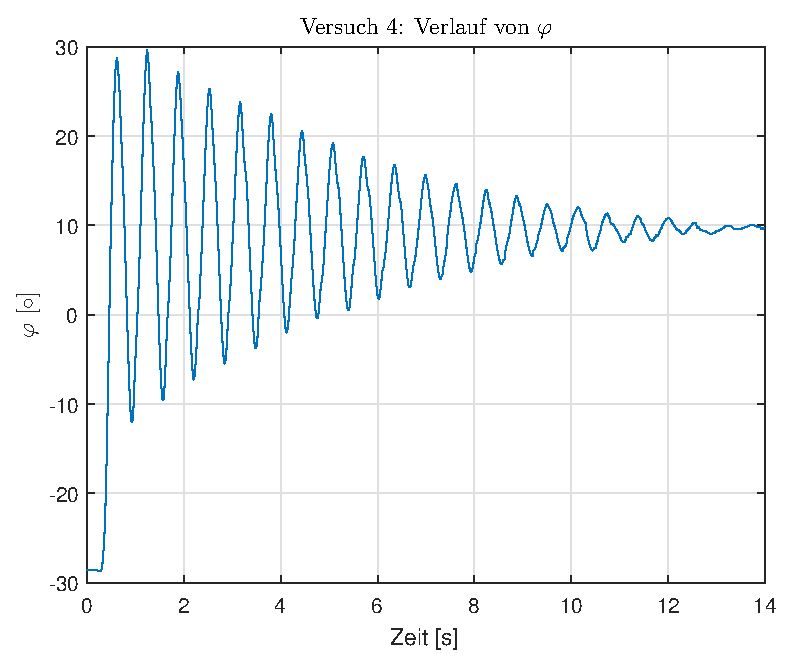
\includegraphics[width=0.5\linewidth]{img/V4_phi.eps}
	\caption{Ausfallwinkel der Würfelseite bei Versuch 4, Quelle: eigene Darstellung}
\end{figure}

Über die $n$ Messpunkte ergeben sich die folgenden Vektoren.

\begin{equation}
\boldsymbol{\varphi} = \begin{pmatrix} \varphi_1 \\ \varphi_2 \\ \vdots \\ \varphi_n \end{pmatrix} \hspace{35pt}
\boldsymbol{\dot{\varphi}} = \begin{pmatrix}
\dot{\varphi_1} \\ \dot{\varphi_2} \\ \vdots \\ \dot{\varphi_n}
\end{pmatrix} \hspace{35pt}
\boldsymbol{\ddot{\varphi}} = \begin{pmatrix}
\ddot{\varphi_1} \\ \ddot{\varphi_2} \\ \vdots \\ \ddot{\varphi_n}
\end{pmatrix}
\end{equation}

Damit ergibt sich durch Umstellen von \ref{ermittlung_c_phi_equation} die folgende Gleichung.

\begin{equation}
C_{\varphi} \cdot \boldsymbol{\dot{\varphi}} = g(m_K \cdot l_{AC} + m_R \cdot l_{AB})sin(\boldsymbol{\varphi}) - (\theta^A_K + \theta^B_R + m_R  \cdot l_{AB}^2) \boldsymbol{\ddot{\varphi}}
\end{equation}

Mit Hilfe der Methode der kleinsten Fehlerquadrate kann nun der Reibwert $C_{\varphi}$ bestimmt werden.

\begin{equation}
C_{\varphi} = 6.2 \cdot 10^{-3} \cdot kg \cdot m^2 \cdot s^{-1}
\end{equation}

